%Last page
\newpage
\scriptsize{
\paragraph{Résumé :}
Les forêts tropicales font face à de nombreuses perturbations qui représentent la troisième source mondiale d’émission de gaz à effet de serre. La déforestation et la dégradation des forêts tropicales sont responsables de l’émission de 8.26 milliards de tonnes de dioxyde de carbone par an (Pearson et al. 2017). La déforestation a retenu l’attention mondiale, mais la dégradation des forêts représente 20\% des émissions de l’Amazonie brésilienne (Asner et al. 2005). La gestion durable des forêts a été proposée comme réponse à la déforestation et la dégradation, malgré la remise en question de la durabilité de l’exploitation forestière (Zimmerman \& Kormos 2012). D’autre part, les forêts tropicales abritent plus de la moitié de la biodiversité terrestre mondiale (Scheffers et al. 2012). Par conséquent, nous avons décidé d’étudier le rôle de la biodiversité dans la réponse des écosystèmes forestiers aux perturbations, en reliant diversité et fonctionnement de l’écosystème (Loreau 2010). Nous avons utilisé l’hypothèse que lors d’une perturbation, grâce à une productivité plus forte, une forêt plus diverse aura une meilleure résilience, en se basant sur la relation positive entre biodiversité et productivité. Nous avons relié cette hypothèse aux effets de complémentarité et de sélection (Loreau \& Hector 2001b). La complémentarité est la combinaison de la partition des ressources et de la facilitation, alors que l’effet de sélection est le résultat de la sélection compétitive. Nous avons ainsi centré l’étude sur les mécanismes impliqués dans la relation entre biodiversité et résilience des écosystème forestiers par une approche par simulation afin d’appréhender les processus à long terme. Nous avons utilisé le modèle TROLL (Maréchaux \& Chave) pour simuler 60 forêts matures aux diversités taxonomiques et fonctionnelles croissantes. Nous avons perturbé toutes les forêts et mesuré la résilience de leurs fonctions écosystémiques. En outre, nous avons mesuré la résilience de l’effet net de la biodiversité que l’on a décomposé en en effets de complémentarité et de sélection. Nous avons trouvé que la diversité améliore la résilience des forêts tropicales, particulièrement au travers de la diversité et l’équitabilité fonctionnelle. De plus, nous avons montré que la complémentarité entre les espèces assurait la résilience de la forêt en début de succession avant de laisser place à l’effet de sélection. Nos résultats suggèrent la possibilité d’une gestion durable des forêts tropicales grâce à une meilleure résilience avec une plus haute diversité. Mais cette conclusion n’a de sens que si l’exploitation sélective est durable (Zimmerman \& Kormos 2012). Au contraire, une gestion non durable des forêts tropicales entraînera des rétroactions négatives diminuant lentement la diversité et donc la résilience des forêts, aboutissant ultimement à la dégradation des forêts.
\paragraph{Mots clés :} Résilience, Biodiveristé, Exploitation sélective, Fonctionnement de l'écosystème
\paragraph{Abstract:}
Forest disturbances are the third worldwide source of greenhous gas. Tropical deforestation and degradation emit 8.26 billion of tons of carbon dioxyde per year (Pearson et al. 2017). Deforestation has retained much attention, but degradation from forest represents 20\% of emissions in brazilian Amazon (Asner et al. 2005). Sustainable forest management has been promoted as an answer to deforestation and degradation, besides logging sustainability has been questionned (Zimmerman \& Kormos 2012). On the other hand, tropical forest host over half of the Earth’s biodiversity (Scheffers et al. 2012). Consequently, we decided to study the role of biodiversity in forest ecosystem answer to disturbance, linking diversity to ecosystem functionning (Loreau 2010). We used the hypothesis that when a disturbance event happen, due to a higher productivity, a more diverse forest will be more resilient, based on the positive relationship between biodiversity and productivity. We linked that hypothesis to the complementarity and selection effects (Loreau \& Hector 2001b). Complementarity is the addition of ressource partitionning and facilitation, whereas selection effect is the result of competitive selection. We thus focused on mechanisms involved in the relationship between biodiversity and forest ecosystem resilience with a simulation approach to assess long term processes. We used TROLL model (Maréchaux \& Chave) to simulate 60 matures forests with growing taxonomic and functional diversities. We disturbed all forests and measured the resilience of their ecosystem functions. Additionnally, we measured biodiversity net effect resilience partitioned into complementarity and selection effects. We found that diversity improved tropical forest resilience, particularly through functional diversity and eveness. Moreover, we showed that complementarity between species insured forest recovery in the beginning of the succession before being replaced by selection effect. Our results suggest the possibility for a sustainable management of tropical forest due to an increased resilience with an higher diversity. But this conclusion has meaning only if selective logging meet sustainability (Zimmerman \& Kormos 2012). On the contrary, unsustainable tropical forest management will lead to negative feedbacks slowly diminishing diversity and thus forest resilience, resulting ultimately in forest degradation.
\paragraph{Keywords:}Resilience, Biodiversity, Selective logging, Ecosystem functionning
}

\vspace*{\fill}
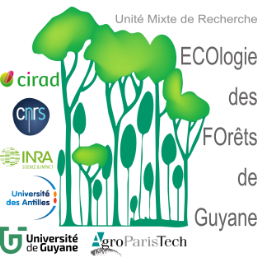
\includegraphics{images/logo}